%-----------------
% Header
%-----------------
\documentclass[
a4paper,                % Papierformat A4frg
12pt,										% Schriftgr��e 12pt
oneside, 								% Zweiseitiges Layout [oneside]
titlepage,              % Titleseite verwenden
headsepline,            % Trennlinie zum Seitenkopf Bereich headings
bibliography=totoc,     % Das Literaturverzeichnis in den TOC
listof=totoc, 					% alle Listen in das Inhaltsverzeichnis
cleardoublepage=plain
% abstractoff,
% appendixprefix=true,		
% headings=normal,      % kleinere �berschriften verwenden
% chapterprefix=false,  % Einf�gen von "Anhang" bzw. "Kapitel" in �berschrift
% plainheadsepline,     % Trennlinie zum Seitenkopf Bereich Plain
% parskip=half-         % Abstand nach Absatz
]{scrbook}


\bibliographystyle{alphadin}

%-----------------
% Packages
%-----------------
\usepackage[ngerman]{babel}
\usepackage{textcomp}
\usepackage[T1]{fontenc}
\usepackage[latin1]{inputenc}
\usepackage{lmodern}
\usepackage{lscape}
\usepackage{rotating}
\usepackage{tocbasic}
\usepackage{color}
%\usepackage{palatino}
%\usepackage{mathpazo}
%\usepackage{courier}
% left = innen, right = au�en
\usepackage[a4paper, left=4cm, right=3cm, top=4cm, bottom=4cm]{geometry} 

\usepackage{graphicx, amsmath, longtable, booktabs, color, listings, makeidx, pdfpages, subfigure}
\usepackage{float}
\usepackage[pdftex,
	hyperindex=true,
	plainpages=false,
	hypertexnames=true,
	bookmarks=true,
	bookmarksnumbered=true,
	pdfhighlight=/O,
	linkcolor=black,
	citecolor=black,
	filecolor=black,
	menucolor=black,
	urlcolor=black,
	colorlinks=true,
	pdftitle={Elektronische Patientenkarte},
	pdfauthor={Alexander Miller},
	pdfsubject={MAGW, Angewandte Informatik},
	pdfstartpage=1]{hyperref}
	
\hyphenation
{
	soft-ware-m�-�i-gen
	kryp-to-gra-phi-schen
	kryp-to-gra-phi-scher
	Ein-weg
	Hash-funk-ti-o-nen
	Pro-to-kol-le
}
	
% Formatierung f�r Code-Listings setzen:
\lstset{basicstyle=\scriptsize\ttfamily,
		keywordstyle=\bfseries\color[rgb]{0.07, 0.21, 0.45},
		keywordstyle=[2]\color[rgb]{0.3, 0.4, 0.5},
		commentstyle={\color[gray]{0.5}\textit},
		stringstyle={\textit},
		xleftmargin=0.5cm, xrightmargin=0cm, framerule=1pt,
		showstringspaces=false, breaklines=true, breakatwhitespace=true,
		numbers=left, numberstyle=\tiny, stepnumber=1, numbersep=0.2cm,
		frame=lines,
		aboveskip=\bigskipamount, belowskip=\bigskipamount,
		framexleftmargin=0.5cm,
		tabsize=4,
		escapeinside={<ref>}{</ref>}}
%--------------------------------------
%   Metainformation
%--------------------------------------
\newcommand{\art}{Mobile Anwendungen im Gesundheitswesen}
\newcommand{\titel}{Elektronische Patientenkarte}
\newcommand{\untertitel}{\empty}
\newcommand{\autor}{Christian Bunk,\\Alexander Miller,\\Benjamin Oertel,\\Christian Sandvoss}
\newcommand{\registriernr}{Mobile Anwendungen im Gesundheitswesen}
\newcommand{\hochschule}{Hochschule f�r Technik und Wirtschaft Berlin}
\newcommand{\fachgebiet}{Angewandte Informatik}
\newcommand{\erstgutachter}{Thorsten Knape}
\newcommand{\datum}{Abgabedatum: 15.01.2012} % durch Abgabedatum zu ersetzen
\newcommand{\ort}{Berlin}


	
%--------------------------------------
%   Dokumentenbeginn
%--------------------------------------
\begin{document}

%--------------------------------------
%   Titelseite
%--------------------------------------
\begin{titlepage}
	\pdfbookmark[-1]{\titel}{Marke}
	% Titelblattkopf
	\titlehead{
		\begin{flushright}
			
\includegraphics[width=0.4\textwidth]{images/HTW_Logo_rgb.jpg}
		\end{flushright}
	}
	
	\subject{Hochschule f�r Technik und Wirtschaft Berlin \\ Angewandten Informatik\\ \large{\mdseries{\registriernr}}} % Art der Arbeit
	\title{\titel}% Titel der Arbeit
	\subtitle{\untertitel}% ggf. Untertitel
	\author{\autor}% Verfasser
	\date{\datum}% Datum
	\publishers{\erstgutachter }% Betreuer
	\maketitle %erzeugt die Titelseite
\end{titlepage}

%--------------------------------------
%   Seitennummerierung
%--------------------------------------
\pagenumbering{Roman}

%--------------------------------------
%   Abstract und Kurzfassung
%--------------------------------------
\newpage

%Inhaltsverzeichnis:
\tableofcontents
%\addcontentsline{toc}{chapter}{Inhaltsverzeichnis}
%Abbildungsverzeichnis:
\listoffigures
%\addcontentsline{toc}{chapter}{Abbildungsverzeichnis}
%Tabellenverzeichnis:
\listoftables
%\addcontentsline{toc}{chapter}{Tabellenverzeichnis}
%Listingverzeichnis:
%\lstlistoflistings
%\addcontentsline{toc}{chapter}{Listingsverzeichnis}


\chapter*{Abk�rzungen}
\label{sec:Abk�rzungen}
\begin{longtable}{l@{\hspace{0.5cm}}p{0.75\textwidth}} \toprule
Abk�rzung          	& Bedeutung\\ \midrule
SQL                 & Structured Query Language\\
\bottomrule
\end{longtable}

\cleardoublepage

%Danksagung:
%\chapter*{Danksagung}
%\label{sec:Danksagung}




\pagenumbering{arabic}

\chapter{Einleitung}
\label{sec:Einleitung}

\section{Motivation und Problemstellung}
\label{sec:Motivation und Problemstellung}

...

\section{Struktur der Arbeit}
\label{sec:Struktur der Arbeit}

...




\chapter{Entwicklung eines Prototyps}
\label{sec:Entwicklung eines Prototyps}

Im Folgenden wird das ausgew�hlte Anwendungsszenario vorgestellt, welches ganzheitlich einen Arbeitsprozess der elektronischen Patientenkarte mit all seinen Teilschritten und m�glichen Anwendungsf�llen ausf�hrlich beschreibt. F�r diesen Zweck erfolgt eine Anforderungsanalyse, die sowohl auf die Ermittlung der einzelnen Personas als auch auf die Spezifikation der User-Interface ausgerichtet ist. Durch die Konzeption und Entwicklung der mobilen Applikation wird es bestrebt eine professionelle Behandlung sowie eine hochqualitative Betreuung f�r alle Patienten zu erm�glichen und dadurch die Kundenzufriedenheit zu erh�hen.

\section{Szenario}
\label{sec:Szenario}

Nach einer administrativen Patientenaufnahme in einem Krankenhaus, weden die Patienten medizinisch behandelt und w�hrend des ganzen Aufenthalts pflegerisch betreut. F�r die Dauer der station�ren Anwesenheit erh�lt jeder Patient ein Armband (RFID-Tag), welcher die eindeutige Identifikation gew�hrleistet. Anschlie�end erfolgt die Erstellung eines neuen Profils, wobei notwendige Stammdaten (Armband-ID, Vorname, Nachname, Geschlecht, Geburtsdatum) sowie die optionale Daten (Gr��e, Gewicht) vom Krankenhauspersonal erfasst und gespeichert werden. Das medizinische Personal, welches f�r die Behandlung der Patienten zugelassen ist, werden mit jeweils einem Tablet ausgestattet. Nach der erfolgreichen Patientenidentifizierung (RFID-Tag auslesen) stehen auf dem Tablet folgende Funktionalit�t zur Verf�gung:

\begin{itemize}
	\item \textbf{Allgemeine Informationen:} Durch die Auswahl dieser Funktion, stehen vielf�ltige Informationen zur Verf�gung. So zum Beispiel besteht die M�glichkeit aktuelle Krankenhausmeldungen oder die online-Speisekarte anzusehen und den betroffenen Patienten zu informieren. 
	\item \textbf{Messung der Vitalfunktionen (K�rpertemperatur):} Nach der Aktivierung dieser Funktion wird die K�pertemperatur mit einem meizinischen Fieberthermometer gemessen und �ber Bluetooth-Funktechnologie an das mobile Ger�t �bertragen. Die erfasten Messdaten werden sowohl lokal auf dem Ger�t gespeichert als auch zu der zentralen Krankenhaus-Datenbank weitergeleitet.
	\item \textbf{Visualisierung der Daten:} Die erfassten Daten k�nnen f�r eine medizinische Analyse visualisiert werden. Dabei werden die Grenzbereiche gekennzeichnet, so dass der Fortschritt sowie die Tendenz der Genesung sich herauskristallisieren. Durch die Auswahl eines Zeitraums werden die Daten in Form eines Diagramms dargestellt und erm�glichen einen schnellen �berblick der einzelnen Vitalfunktionen.
\end{itemize}

Damit der Vergleich von gemessenen Werten ein repr�sentatives Ergebnis bereitstellt, ist es erforderlich die einzelnen Vitalfunktionen t�glich um 08:00, 16:00 und 20:00 zu messen. Dabei muss es immer �berpr�ft werden, dass die Messung korrekt durchgef�hrt wird und die Messwerte in einem akzeptablen Bereich (z.B. 27 �C - 42,8 �C) liegen. F�r die p�nktliche Messung sorgt die Erinnerungsfunktion, welche mit Hilfe von akustischen Signalen das zust�ndige Personal an die bevorstehende Messung rechtzeitig aufmerksam macht. 

Eine clientseitige Webanwendung erm�glicht sowohl f�r �rzte als auch f�r die Patienten eine Betrachtung der gemessenen Daten. Durch die Festlegung der Wertebereiche sowie die automatisierte Anaylsen, werden die Patienten mit kritischen Messwerten informiert und f�r die priorisierte Behandlung gekennzeichnet.

\section{Anforderungsanalyse}
\label{sec:Anforderungsanalyse}

F�r die Realisierung eines Projekts dieser Gr��e, ist es erforderlich die einzelnen Systemkomponente zu kennzeichnen sowie den Informationsfluss darzustellen. Wie in der Abbildung \ref{fig:Systemaufbau} dargestellt �bernimmt das mobile Ger�t die Funktionalit�t einer Komunikationsschnittstelle zwischen dem NFC f�higen medizinischen Ger�t und dem Server. Die clienseitige Anwendung erm�glicht die Visualisierung sowie die anschlie�ende Analyse der erfassten Daten und erm�glicht einen Fernzugriff auf die erforderliche Informationen.

\begin{figure}[ht]
\centering
		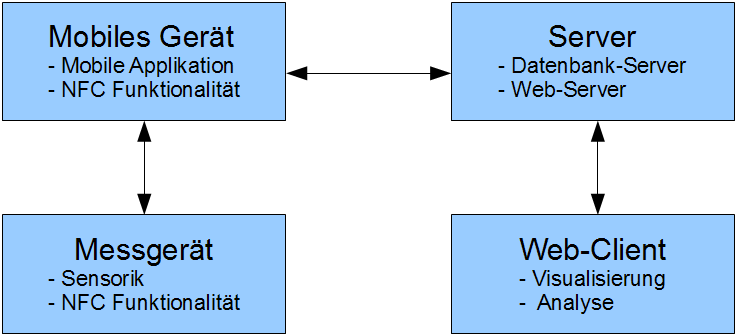
\includegraphics[height=4.5cm]{images/Systemaufbau.png}
	\caption[Systemaufbau] {Systemaufbau}
	\label{fig:Systemaufbau}
\end{figure}

Folgende technische Komponenten stehen f�r die Entwicklung zur Verf�gung:
\begin{itemize}
	\item Messger�t: Arduino Board + NFC-Shield + Temperatursensor
	\item Mobiles Endger�t: Samsung Nexus S
	\item Web-Server an der Hochschule f�r Technik und Wirtschaft Berlin
\end{itemize}

\section{Konzeption und Implementierung}
\label{sec:Konzeption und Implementierung}

...
\chapter{Fazit}
\label{sec:Fazit}

...
%Literaturverzeichnis:
%\bibliography{C:/literatur}

%% Anh�nge:
%\appendix
%
%\chapter{Anhang}
%\label{sec:Anhang}
%
%\section{Aufgabenstellung}
%\label{lst:Aufgabenstellung}
%
%...
%
%\chapter{Quelltext}
%\label{sec:Quelltext}
%
%\section{Projekt}
%\label{sec:Projekt}
%\lstset{language=C++}
%\lstinputlisting[ caption={[Projekt] Projekt }, captionpos=t]{Listings/Projekt.c}
%\clearpage


%--------------------------------------
%   Dokumentenende
%--------------------------------------
\end{document}
